\documentclass[../relazione.tex]{subfiles}

\begin{document}
\section{Progettazione}
	In seguito sono riportate in forma di elenco tutte le scelte progettuali effettuate durante lo sviluppo del progetto che il gruppo ha ritenuto degne di nota, suddivise per ambito di interesse: \texttt{XHTML}, \texttt{CSS}, \texttt{Perl/CGI}, \texttt{Javascript}, \texttt{XML} e \texttt{XMLSchema}.\\
	Tutte le scelte che riguardano puramente la parte mobile sono state riportante a parte nella sezione 5.6 \textit{Mobile} del presente documento.
	\subsection{XHTML}
	\begin{itemize}
		\item Il logo del sito è stato realizzato con una \texttt{background-image} sfruttando la tecnica di \textit{image replacement} affinché possa costituire informazione per il motore di ricerca.
		\item Nella parte pubblica del sito, il \texttt{path} svolge sia funzione di breadcrumb che di titolo della pagina: avendo un solo livello profondità, abbiamo ritenuto non necessario il breadcrumb all'interno della parte pubblica del sito.
		\item Per indicare al motore di ricerca l'importanza dei termini caratteristici del ristorante e della cucina giapponese è stato usato \texttt{strong}: questa è un'operazione di SEO (\textit{Search Engine Optimization}).
		\item La struttura di ogni pagina è stata pensata per evidenziare le informazioni che si ritengono più importanti per un utente che naviga su un sito di ristorazione. Quindi si è deciso di tenere in alto e visibile in maniera chiara in ogni pagina della parte pubblica del sito i seguenti elementi:
		\begin{itemize}
			\item il \textit{luogo} dove si trova il ristorante, che è un'ancora a \texttt{dove-siamo.html}: una pagina che presenta informazioni più dettagliate sulla posizione del ristorante
			\item il \textit{numero di telefono}, che è un'ancora alla funzione di inizio della telefonata (\texttt{tel:})
		\end{itemize}
		\item Nella pagina \texttt{index.html} sono stati messi in evidenza l'\textit{orario}, le \textit{informazioni generali} riguardo il ristorante e la possibilità di usufruire del servizio di \textit{take away}.
		\item Per fidelizzare il cliente, nella pagina \texttt{chi-siamo.html} mostriamo le personalità principali che gestiscono l'attività, come il proprietario del ristorante e i cuochi, raccontando un sunto del loro curriculum o le loro esperienza passate nel campo della ristorazione.
		\item Nella pagina \texttt{dove-siamo.html} è presente una breve descrizione testuale di dove si trova il ristorante accompagnata da un'immagine che ne indica la posizione rispetto ai vicini punti di interesse. Per rendere accessibile l'immagine a chi utilizza uno screen reader è stato utilizzato l'attributo \texttt{longdesc} che associa una descrizione testuale dettagliata (definita nel file \texttt{indicazioni.txt}) all'immagine. Oltre a questo, è presente un link a Google Maps per agevolare l'utente nella ricerca di indicazioni precise per raggiungere il ristorante: nel caso in cui stia navigando da un dispositivo mobile ed abbia l'applicazione di Google Maps installata, verrà automaticamente lanciata l'applicazione.
		\item Nella pagina \texttt{curiosita.html} abbiamo inserito una serie di curiosità sulla cucina giapponese per far conoscere all'utente un po' della sua storia.
		\item Tutti i nomi delle pietanze nella pagina \texttt{menu.cgi} sono inseriti in un tag \texttt{strong} per indicarne l'importanza al motore di ricerca: questa è un'operazione di SEO (\textit{Search Engine Optimization}).
		\item L'area amministratore permette di aggiungere, modificare o rimuovere pietanze o bevande dal menù.
	\end{itemize}
	\subsection{CSS}
	\begin{itemize}
		\item Si è cercato di utilizzare meno colori possibili.
		\item Si è scelto di utilizzare i colori di bandiera del ristorante, ricavati dal logo fornitoci dal proprietario del ristorante.
		\item Tali colori sono stati scelti antagonisti, per venire incontro a utenti con problemi di colorblindness ed aumentando così l'accessibilità del sito.
		\item Lo sfondo in legno dell'intero sito web vuole ricordare la stuoia usata nel processo di creazione del sushi e, più in generale, lo stile nipponico.
		\item Si è deciso di non inserire nel \texttt{footer} del sito l'icona di validazione ottenuta dal W3C in quanto non in linea con i colori del layout. Il sito è stato comunque interamente validato sia nel CSS che nel XHTML.
		\item Al foglio di stile \texttt{style.css} è stato applicato il \textit{minifier} per un miglioramento delle performance.
		\item Viene fornito anche il file \texttt{style\_extended.css}, che sarebbe il foglio di stile prima dell'applicazione del \textit{minifier}, per migliorare la lettura in fase di correzione del progetto.
	\end{itemize}
	\subsection{Perl/CGI}
	\begin{itemize}
		\item Script in \texttt{Perl/CGI} vengono usati per gestire la visualizzazione dei dati nel database \texttt{XML} e gestire eventuali inserimenti, modifiche e rimozioni su di esso.
		\item Gli script utilizzati vanno ad impattare in entrambe le aree del sito, sia pubblica che privata (Area amministratore).
		\item Gli script \texttt{CGI} sono così suddivisi nella cartella cgi-bin:
			\begin{itemize}
				\item script di pagina riservata al login all'area amministratore;
				\item script di pagine riservate all'accesso pubblico del menù del ristorante;
				\item script di pagine riservate all'accesso dell'amministratore (simile al menù presentato all'utente ma con form e pulsanti aggiunti, questi script sono anche incaricati della rimozione);
				\item script di pagine riservate per l'aggiunta (prefisso \texttt{add-});
				\item script di pagine riservate per la modifica (prefisso \texttt{mod-});
				\item script per effettuare il logout che termina la sessione e reindirizza il browser;
				\item moduli perl all'interno della cartella \texttt{My} che racchiudono le subruotines utilizzate per gli altri script \texttt{Perl/CGI};
			\end{itemize}
		\item Le uniche pagine accessibili senza credenziali sono:
			\begin{itemize}
				\item \texttt{menu.cgi}: crea, prelevando i dati dal database \texttt{XML}, il menù del ristorante;
				\item \texttt{login.cgi}: permette tramite l'inserimento di admin e password l'accesso all'area amministratore.
			\end{itemize}
		\item Si può accedere all'area amministratore tramite login da ogni pagina del sito tramite link situato nel footer. Tutte le pagine della sezione amministrativa che effettuano modifiche in scrittura nel database sono protette da credenziali (riportate in prima pagina della presente relazione). Se corrette verrà visualizzata la pagina \texttt{private-menu-cibi.cgi} per prima. Il \texttt{nav} del sito pubblico sarà sostituito da un \texttt{nav} di sole due sezioni:
			\begin{itemize}
				\item Cibi
				\item Bevande
			\end{itemize}
da cui sarà possibile effettuare le operazioni sul file \texttt{menu.xml}. Si è deciso di separare le due componenti per agevolare il lavoro dell'amministratore perché tutto il menù del ristorante creava una pagina troppo lunga con l'aggiunta di form e pulsanti.
		\item Per far ciò si è ricorso all'utilizzo delle sessioni \texttt{Perl} e relativa libreria. Ogni pagina effettua al caricamento un controllo della sessione aperta e se risulta non valida o scaduta (dopo 60 minuti) l'amministratore o qualsiasi utente che prova l'accesso sono reindirizzati verso la pagina \texttt{accesso-negato.html}. Questa pagina viene mostrata in tutti i casi in cui l'utente o non ha le credenziali o la sessione è scaduta.
		\item Poiché l'area amministrativa conterà un solo amministratore non si è ritenuto necessario l'utilizzo di parametri all'interno della sessione tranne l'username.
		\item Per l'uscita invece sono stati inseriti due link 'uscita' nel top e nel bottom delle pagine che chiudono la sessione e indirizzano alla pagina \texttt{index.html}.
		\item Per poter rimuovere un piatto o una bevanda è sufficiente utilizzare i pulsanti "Rimuovi" situati vicino ogni elemento del menù del ristorante nelle pagine:
			\begin{itemize}
				\item \texttt{private-menu-cibi.cgi}
				\item \texttt{private-menu-bevande.cgi}
			\end{itemize}
			Una volta premuto il pulsante la pagina viene ricaricata e un messaggio ad inizio pagina avverte se tutto è andato a buon fine.
		\item Per poter aggiungere un piatto o una bevanda è necessario effettuare il submit sulle form di aggiungi dalle pagine:
			\begin{itemize}
				\item \texttt{private-menu-cibi.cgi}
				\item \texttt{private-menu-bevanda.cgi}
			\end{itemize}
			perché da esse vengono prelevati i campi \texttt{hidden} necessari al corretto funzionamento dell'inserimento. È possibile aggiungere piatti e bevande ma non portate o liste di bevande (vini, birre, etc.) in quanto già sufficienti a comprendere eventuali piatti o bevande nuove. Non si è comunque escluso che in un futuro questa funzionalità non possa essere aggiunta. Prima di ogni aggiunta i nuovi dati inseriti sono opportunamente controllati tramite espressioni regolari per far sì che il database risulti ben formato e valido secondo il relativo schema.
		\item Per poter modificare un piatto o una bevanda è necessario effettuare il submit sulle form di modifica dalle pagine:
			\begin{itemize}
				\item \texttt{private-menu-cibi.cgi}
				\item \texttt{private-menu-bevanda.cgi}
			\end{itemize}
			perché da esse vengono prelevati i campi \texttt{hidden} necessari al corretto funzionamento della modifica. Le form di modifica sono infatti già compilate con i dati presenti nel file \texttt{menu.xml}. Prima di ogni modifica i nuovi dati inseriti sono opportunamente controllati tramite espressioni regolari per far sì che il database risulti ben formato e valido secondo il relativo schema.
		\item Sono stati scritti in totale tre package \texttt{Perl} con lo scopo di riutilizzare il codice e di renderlo il più possibile manutenibile. Essi dividono le funzioni in base al loro luogo di utilizzo. Di seguito la lista dei package e una descrizione delle funzioni racchiuse all'interno:
			\begin{itemize}
				\item \texttt{Base}: racchiude tutte le funzioni per la stampa dell'\texttt{HTML} più frequente (come ad esempio l'\texttt{header}) e tutte le funzioni per agevolare l'accesso sia in lettura che scrittura sul database \texttt{XML};
				\item \texttt{PrintMenu}: racchiude le funzioni che si occupano della raccolta di dati dal database \texttt{XML} e alla stampa con o senza la presenza di form per l'area amministratore;
				\item \texttt{Operation}: raccoglie tutte le funzioni che costruiscono le form di aggiunta e modifica e controllano che i dati inseriti siano corretti e soprattutto che non invalidino il database.
			\end{itemize}
	\end{itemize}
	\subsection{Javascript}
	\begin{itemize}
		\item Il menu del sito (chiamato d'ora in poi anche \texttt{nav}) è inizialmente visibile, così se \texttt{Javascript} non è attivo il sito ha una degradazione elegante.
		\item Se invece \texttt{Javascript} è attivo e la navigazione viene effettuata da mobile, allora il \texttt{nav} viene nascosto e rimane accessibile dall'apposita \texttt{icon hamburger}.
		\item È presente il controllo tramite \texttt{Javascript} dei dati inseriti nei campi delle form, per segnalare eventuali errori all'utente in maniera immediata, senza attendere una risposta del server.
		\item Nella pagina \texttt{menu.cgi} e \texttt{private-menu.cgi}, il menù è diviso in categorie inizialmente chiuse per diminuire la lunghezza della pagina e dare all'utente una visione generale delle categorie di pietanze e bevande presenti nel menù.
		\item Nel caso in cui il \texttt{Javascript} non sia attivo, il menù verrà mostrato per intero, ma viene aggiunta una funzionalità di ricerca veloce (in alto nella pagina) e, alla fine di ogni categoria, un'ancora per tornare all'inizio della pagina.
	\end{itemize}
	\subsection{XML e XMLSchema}
	\begin{itemize}
		\item Per modellare il menù del ristorante in un database XML si è deciso di fare una forte divisione logica tra cibi e bevande.
		\item Quest'ultimo è presente nella cartella \texttt{data} ed è il documento \texttt{menu.xml}: esso è ben formato e valido secondo lo schema \texttt{menu.xsd}, presente nella stessa cartella.
		\item Il modello scelto per modellare lo schema in \texttt{XMLSchema} è Tende alla Veneziana, in quanto sfrutta i tipi nominali e, basandosi sul menù da modellare, era necessario riutilizzare i tipi definiti in precedenza. 
		\item È stato definito un tipo complesso \texttt{stringWithSpan} per permettere ai nomi (sia delle portate che delle bevande) e alle descrizioni di contenere, nel caso in cui sia presente una parola straniera, un tag \texttt{span} che definisca tramite l'attributo \texttt{xml:lang} la lingua della parola. \texttt{stringWithSpan} permette anche di contenere il tag \texttt{abbr} per le eventuali abbreviazioni.
		\item \texttt{stringWithSpan} è stato definito come un tipo misto contenente una \texttt{xsd:choice} (con \texttt{minOccurs="0"} e \texttt{maxOccurs="unbounded"}) che permetta una scelta tra l'elemento \texttt{span} e \texttt{abbr}.
		\item Il tipo di \texttt{span} è stato definito con un tipo complesso dal contenuto semplice, ricavato per estensione da \texttt{xsd:string} aggiungendo un attributo \texttt{xml:lang} : quest'ultimo fa riferimento all'attributo \texttt{xml:lang} dello schema \texttt{xml.xsd} contenuto in \url{http://www.w3.org/2001/xml.xsd}, quindi è stato necessario importare il namespace "\url{http://www.w3.org/XML/1998/namespace}".
		\item Il tipo di \texttt{abbr} è molto simile al tipo di \texttt{span}, con l'aggiunta di un attributo \texttt{title} che permette di indicare il nome completo della parola abbreviata.
		\item La definizione del tipo \texttt{stringWithSpan} è stata necessaria data l'elevata presenza di parole straniere all'interno del menù da modellare.
		\item È stato definito un tipo \texttt{Tpiatto} che è stato riutilizzato per ogni piatto presente all'interno del menù: ciò è stato possibile impostando \texttt{minOccurs="0"} sugli elementi \texttt{numero} e \texttt{descrizione} presenti al suo interno. Ciò ha permesso di riutilizzarlo in vari contesti.
		\item Ogni tag \texttt{portata}, \texttt{piatto}, \texttt{listaBevande} e \texttt{bevanda} presenta un attributo \texttt{id} che permette di identificarli in maniera univoca.
		\item Il tipo di prezzo è stato definito con un tipo complesso dal contenuto semplice, ricavato per estensione da \texttt{xsd:decimal} aggiungendo l'attributo \texttt{valuta} di tipo \texttt{xsd:string} : questo attributo non si trova nel file \texttt{menu.xml} in quanto è stato definito un valore di default impostato a \texttt{"euro"} e nel caso da modellare non erano presenti altre valute.
		\item Il file \texttt{admins.xml} invece contiene l’username e password per accedere all’area amministratore, prevedendo la possibile aggiunta di ulteriori amministratori in futuro: nella stessa cartella è fornito lo schema secondo cui il documento \texttt{XML} è valido: \texttt{admins.xsd}; lo schema è stato definito anch'esso in \texttt{XMLSchema} seguendo il modello Tende alla Veneziana.
	\end{itemize}
	\subsection{Mobile}
	Una grossa fetta di utenza del sito è composta dai ragazzi più giovani, come dimostrato dall'analisi presente alla sezione 3 \textit{Analisi dell'utenza} del presente documento.
	Per questo motivo il gruppo ha deciso di definire lo stile del sito anche per i dispositivi mobile, tenendo conto che la maggior parte degli accessi al sito da parte di ragazzi giovani verrà effettuata da smartphone o tablet.\\
	Di seguito sono riportate le scelte progettuali effettuate durante lo sviluppo del progetto che il gruppo ha ritenuto degne di nota per quanto riguarda la parte mobile del sito.
	\begin{itemize}
		\item È stata usata la \texttt{hamburger icon} come simbolo del menu del sito (\texttt{nav}), ritenuta adeguata in quanto è ormai una consuetudine per gli utenti associare ad essa il menu del sito.
		\item Per agevolare la visita del sito e rendere più piacevole l'esperienza dell'utente, abbiamo dato all'utente la possibilità di aprire e chiudere il \texttt{nav}: per far ciò è stata utilizzata una funzione \texttt{Javascript} che mostra e nasconde il \texttt{nav} attraverso la \texttt{hamburger icon}.
		\item Abbiamo convenuto che la parte mobile sia dedicata interamente agli utenti esterni, quindi abbiamo impedito l'accesso all'area amministratore da mobile: esso è permesso solo da desktop.
		\item Il sito è stato testato sui seguenti browser mobile: Google Chrome, Safari.
	\end{itemize}
	\begin{figure}[H]
		\centering
		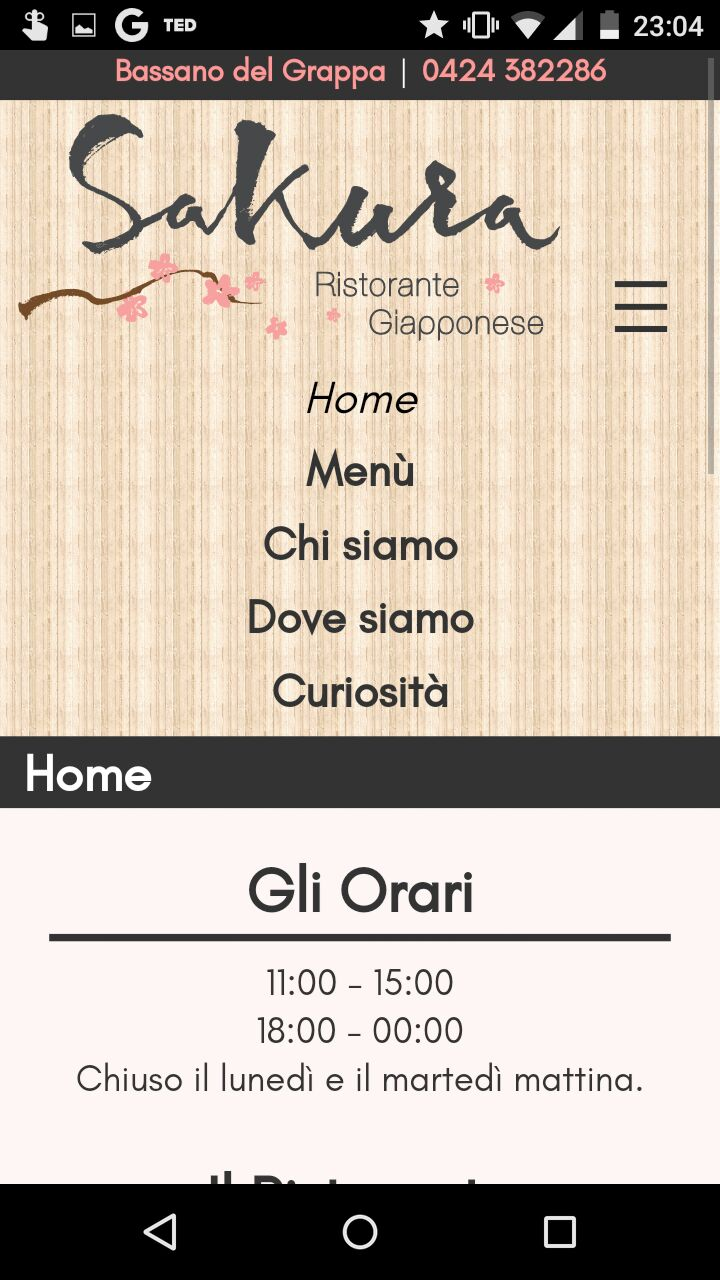
\includegraphics[scale=0.2]{images/mobile2}
		\caption{Esempio di pagina vista da dispositivo mobile con menu a tendina aperto}
		\label{fig:Esempio di pagina vista da dispositivo mobile con menu a tendina aperto}
	\end{figure}
\end{document}